


\section{Question 4}
\label{part1}

\begin{itemize}
\item Choose a news-related event
\item Use twarc.py to collect 1000 tweets, every day for 5 different days
\begin{itemize}
\item See: \url {https://github.com/edsu/twarc}
\end{itemize}
\item For each day:
\begin{itemize}
\item Create a wall
\item Build a tag/word cloud for each day
\item Create a map using GeoJSON \& Github
\begin{itemize}
\item \url {https://help.github.com/articles/mapping-geojson-files-on-github/} 
\end{itemize}
\end{itemize}
\item Discuss in detail lessons learned, experiences, etc.
\end{itemize}
\subsection{Solution}

\begin{itemize}
	\item Installed twarc\cite{jusText} to retrieve 1000 tweets.
	\item I used twarc to build tweets wall, word cloud and to retrieve geojson.
\end{itemize}


\begin{figure}[ht]
	\begin{center}
		 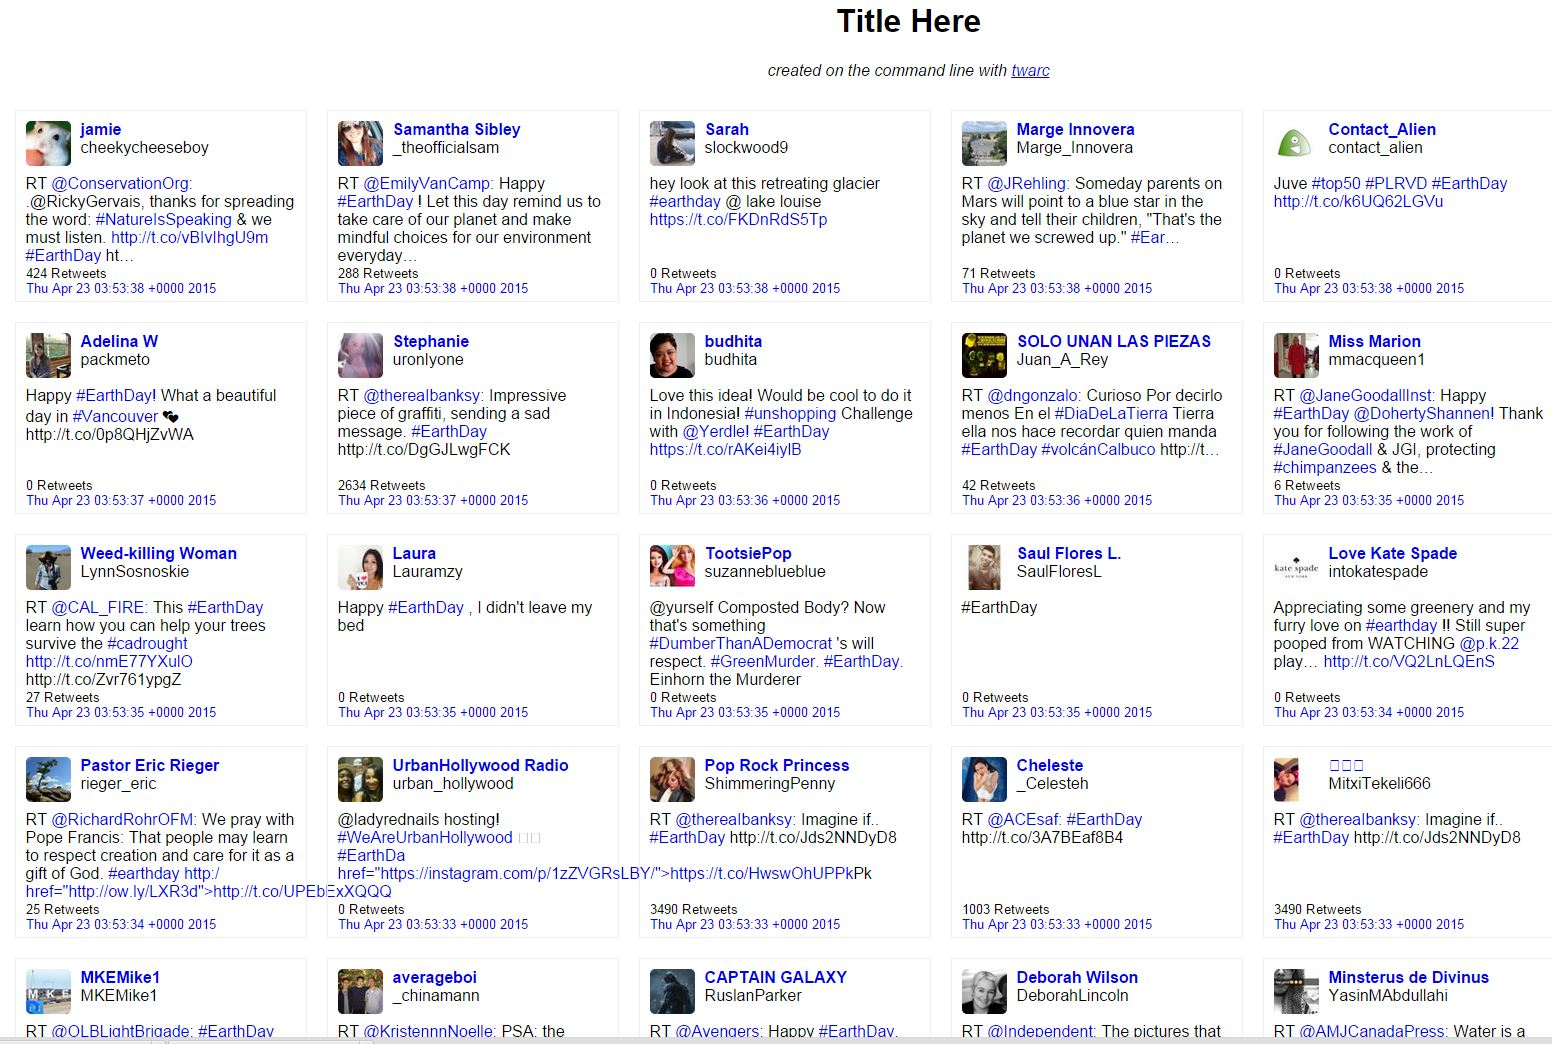
\includegraphics[scale=0.40]{Day1Wall}
		  \caption{Tweets Wall Day1}
	 \end{center}
\end{figure}

\begin{figure}[ht]
	\begin{center}
		 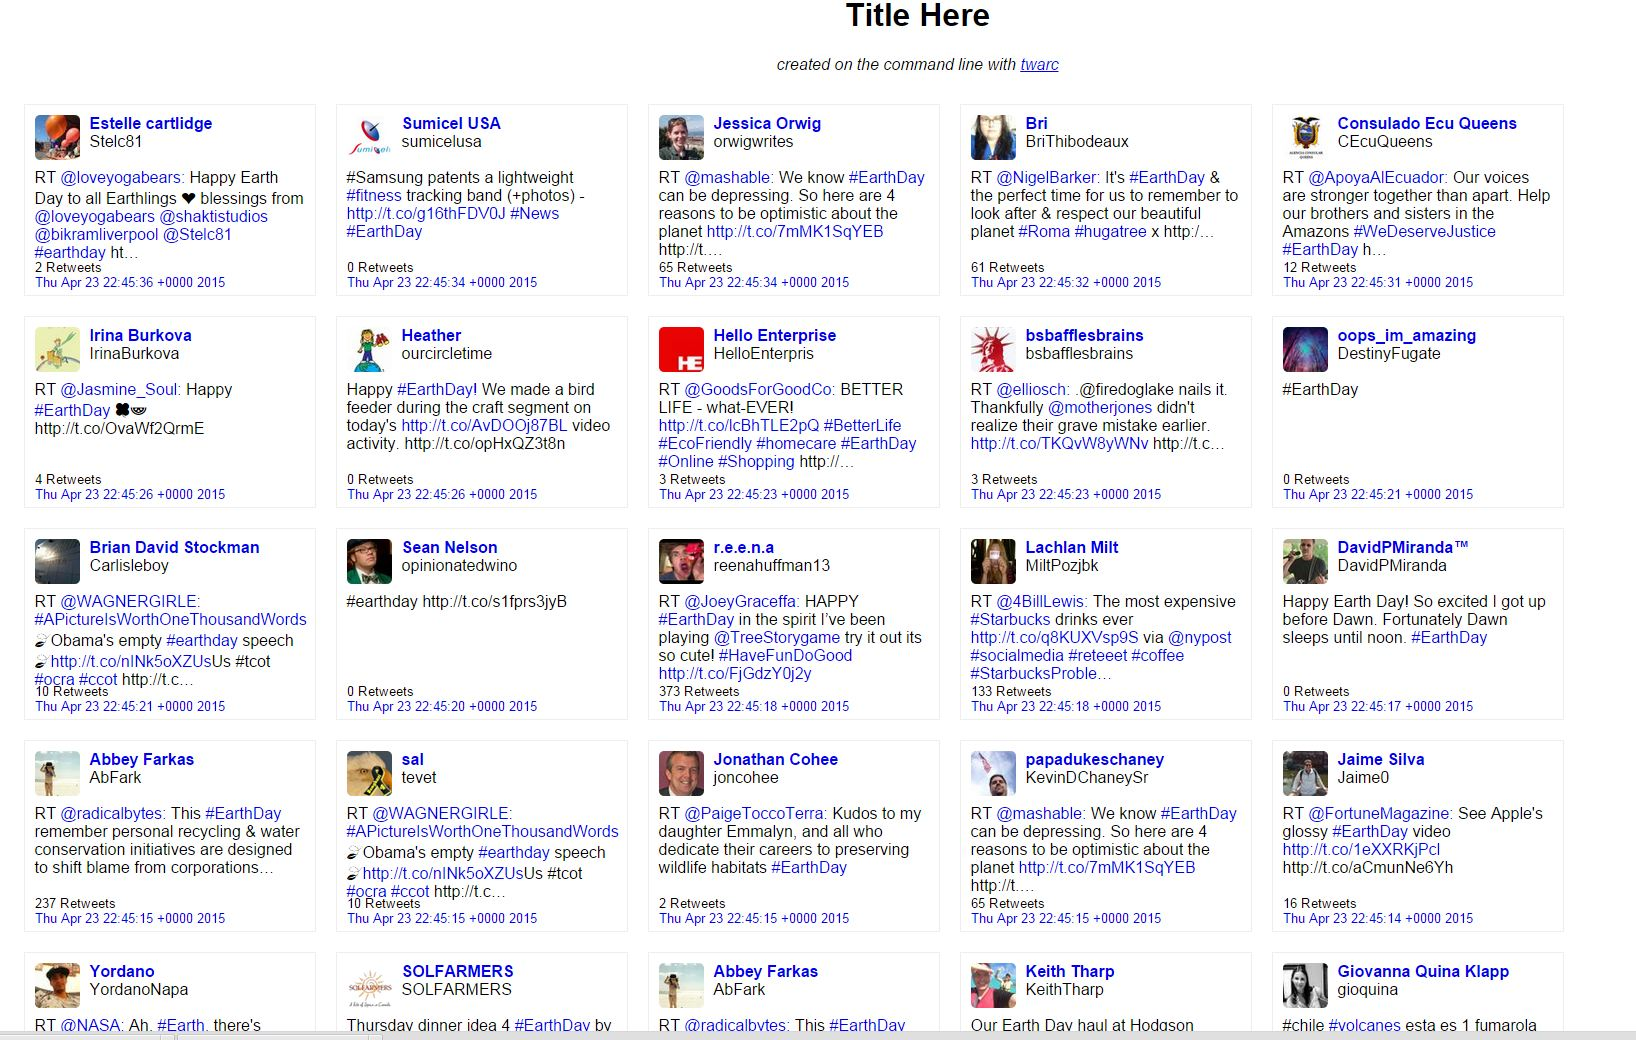
\includegraphics[scale=0.40]{Day2Wall}
		  \caption{Tweets Wall Day2}
	 \end{center}
\end{figure}
\begin{figure}[ht]
	\begin{center}
		 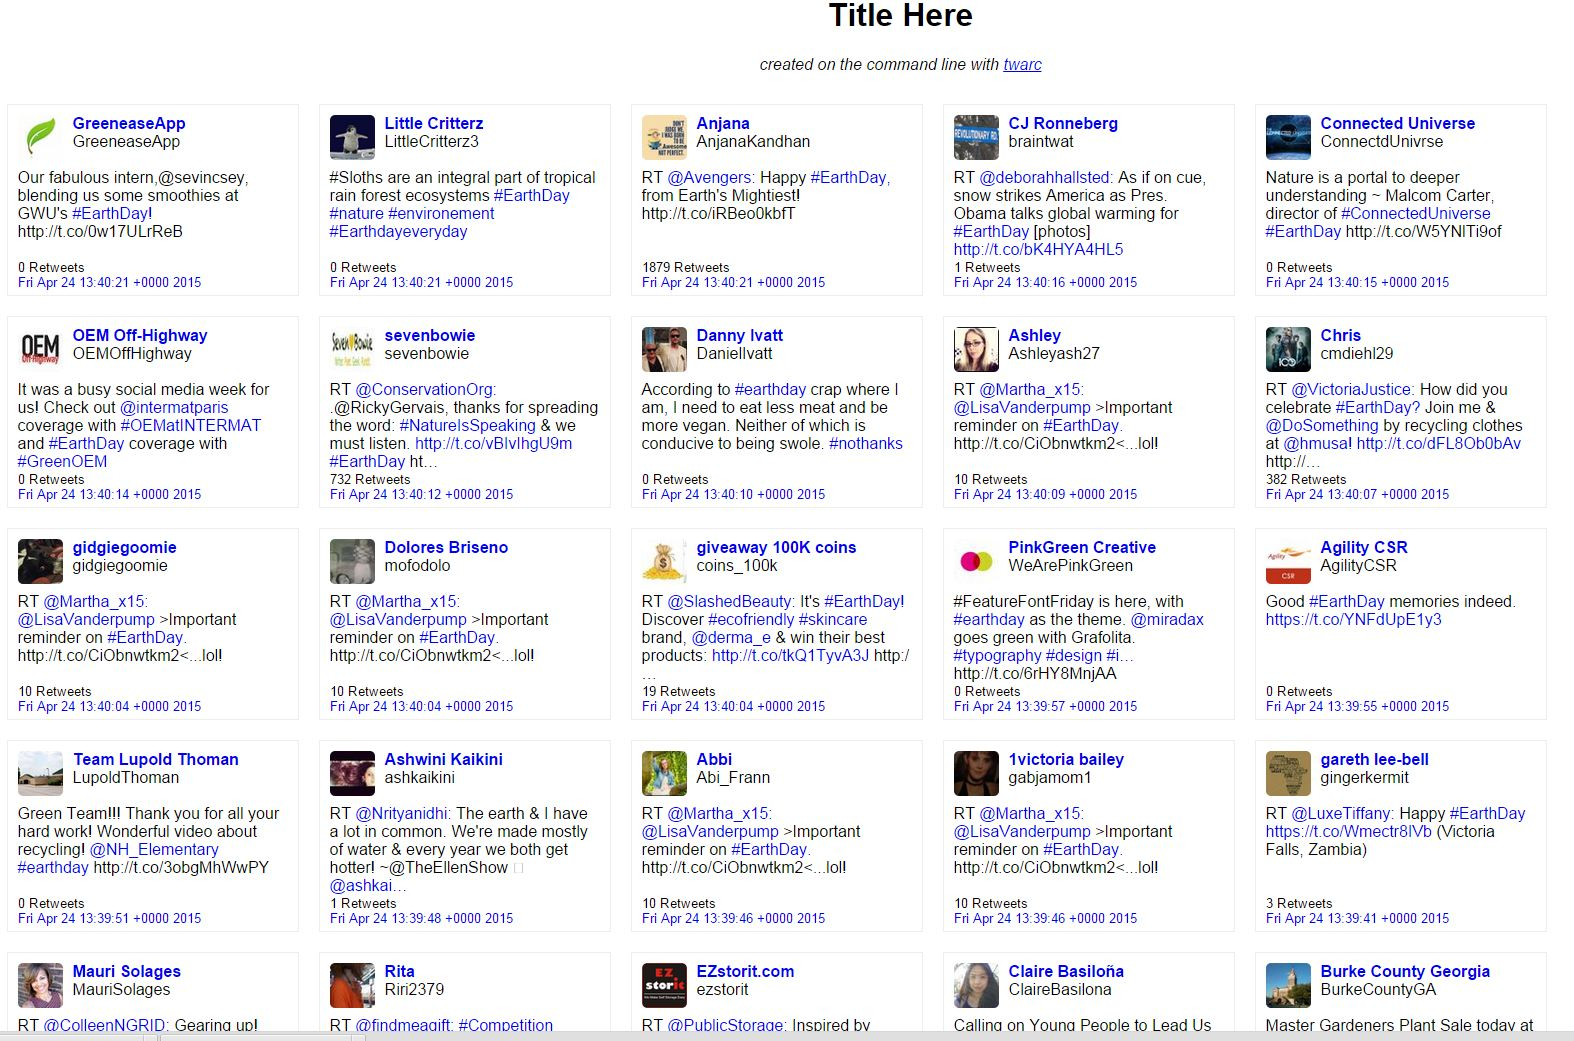
\includegraphics[scale=0.40]{Day3Wall}
		  \caption{Tweets Wall Day3}
	 \end{center}
\end{figure}

\begin{figure}[ht]
	\begin{center}
		 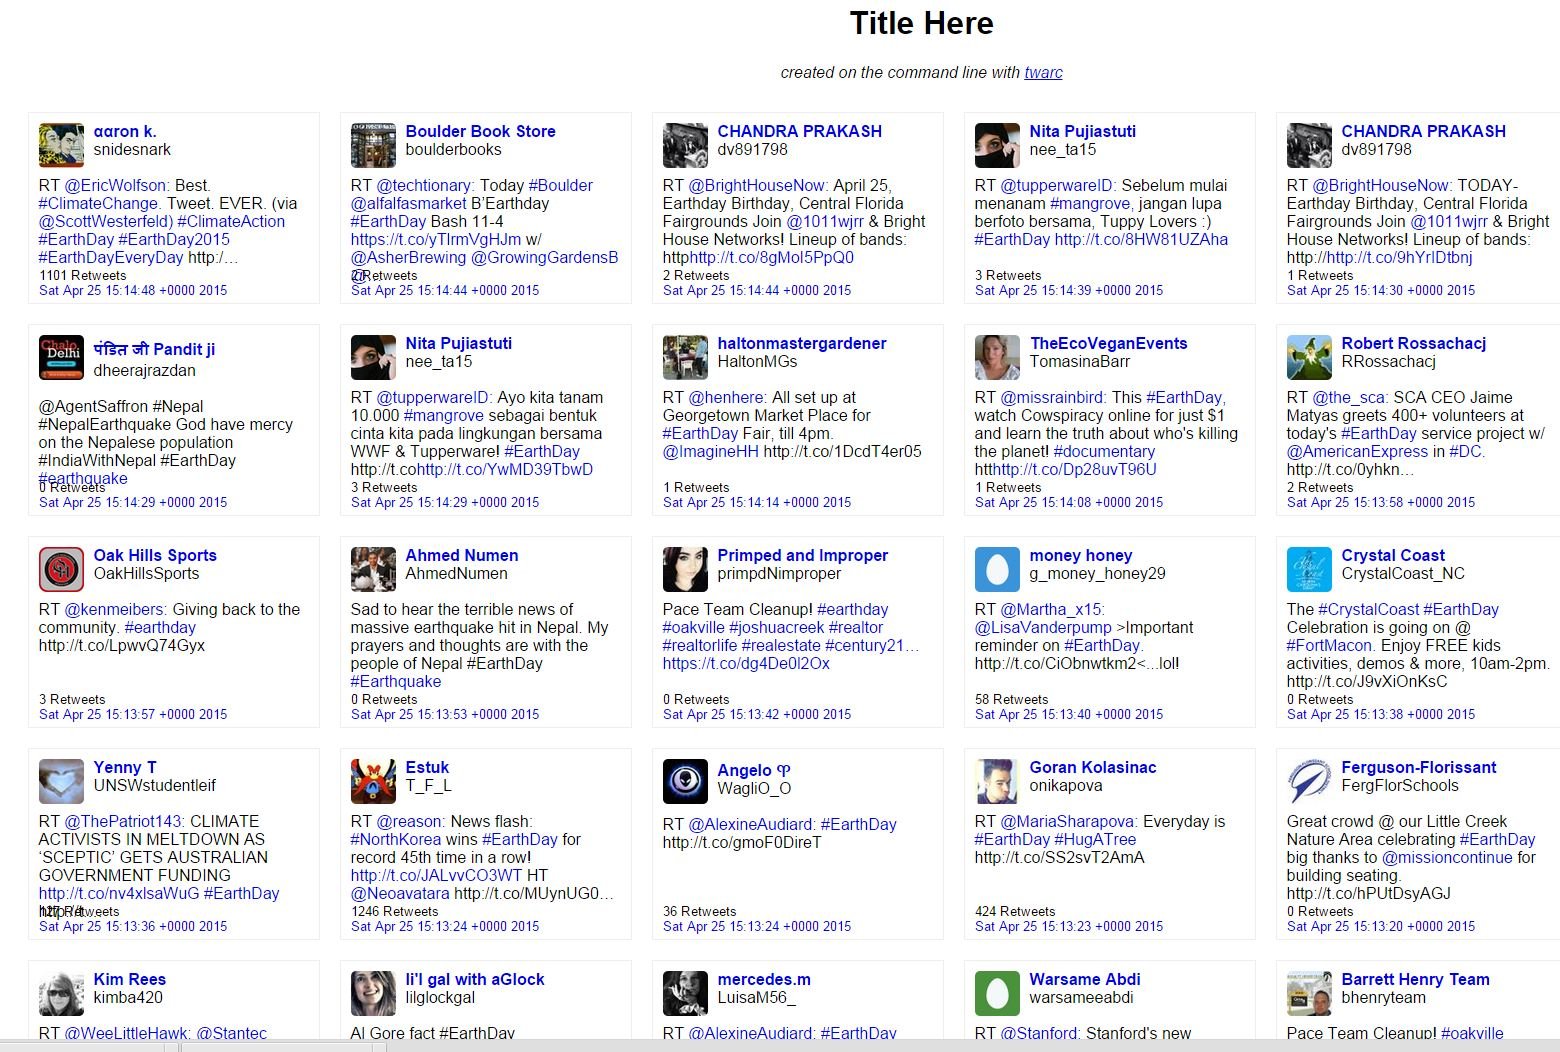
\includegraphics[scale=0.40]{Day4Wall}
		  \caption{Tweets Wall Day4}
	 \end{center}
\end{figure}
\begin{figure}[ht]
	\begin{center}
		 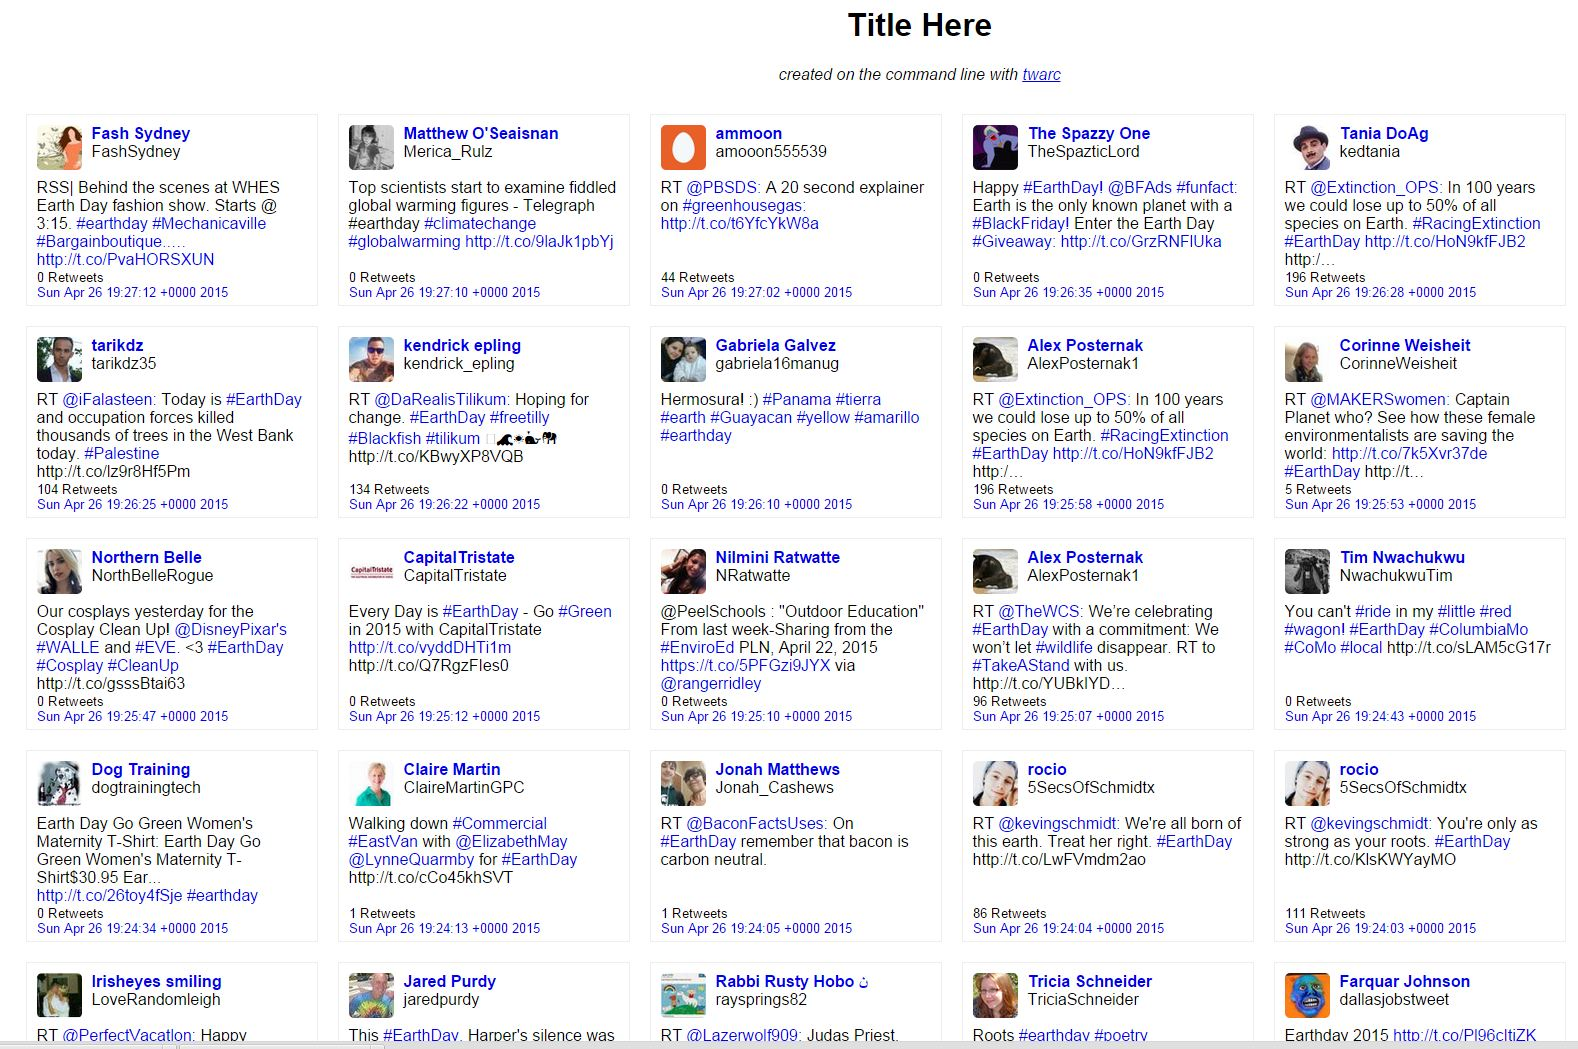
\includegraphics[scale=0.40]{Day5Wall}
		  \caption{Tweets Wall Day5}
	 \end{center}
\end{figure}
\begin{figure}[ht]
	\begin{center}
		 
\includegraphics[scale=0.90]{wordcloudday1}
		  \caption{Tweets Word Cloud Day1}
	 \end{center}
\end{figure}
\begin{figure}[ht]
	\begin{center}
		 
\includegraphics[scale=0.90]{wordcloudday2}
		  \caption{Tweets Word Cloud Day2}
	 \end{center}
\end{figure}
\begin{figure}[ht]
	\begin{center}
		 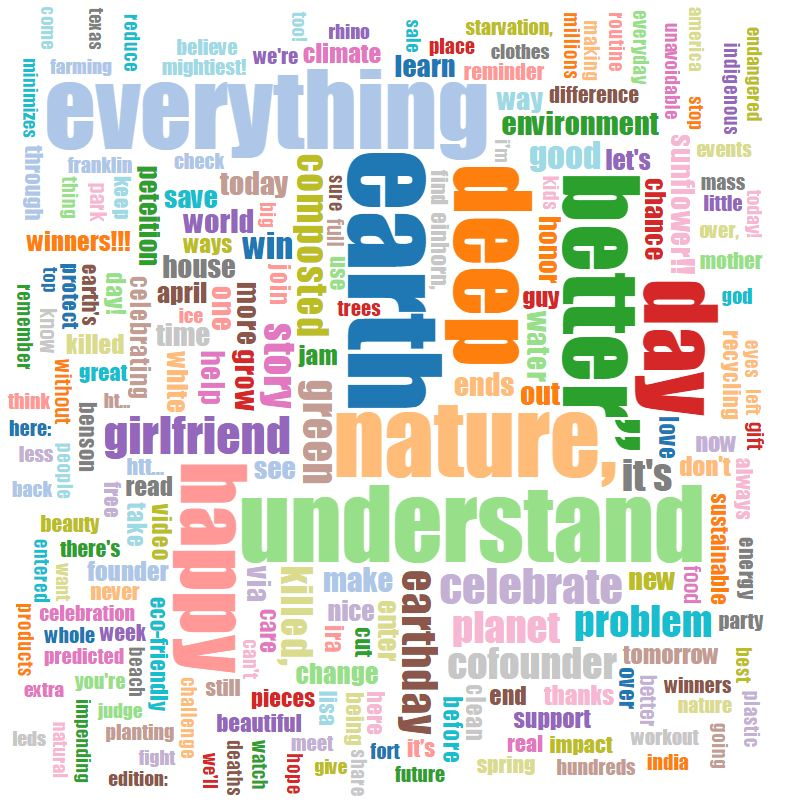
\includegraphics[scale=0.90]{wordcloudday3}
		  \caption{Tweets Word Cloud Day3}
	 \end{center}
\end{figure}
\begin{figure}[ht]
	\begin{center}
		 
\includegraphics[scale=0.90]{wordcloudday4}
		  \caption{Tweets Word Cloud Day4}
	 \end{center}
\end{figure}
\begin{figure}[ht]
	\begin{center}
		 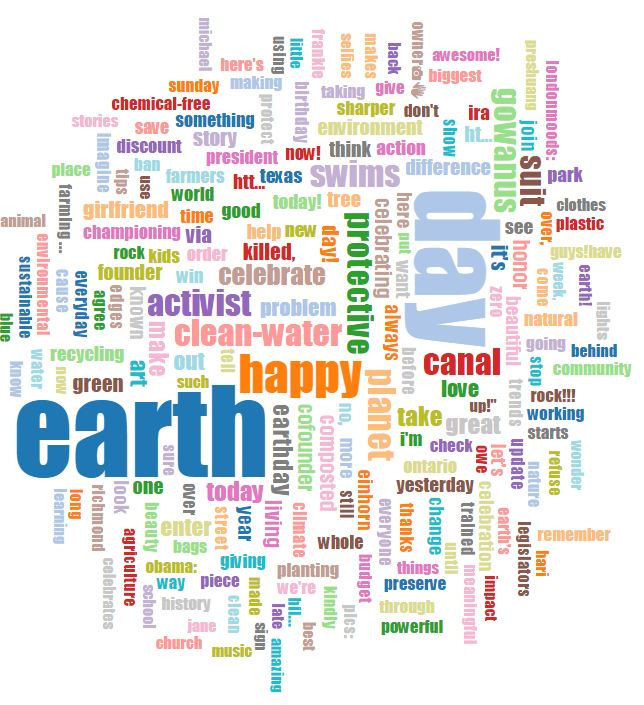
\includegraphics[scale=0.90]{wordcloudday5}
		  \caption{Tweets Word Cloud Day5}
	 \end{center}
\end{figure}

\newpage
